\textbf{b. Instruction Register (IR)}

Instruction Register (Thanh ghi lệnh) đóng vai trò là bộ chốt dữ liệu trung gian 
trong kiến trúc CPU. Nó có nhiệm vụ lưu giữ câu lệnh 32-bit vừa được 
lấy từ bộ nhớ trong giai đoạn Fetch, 
đảm bảo lệnh được giữ ổn định để Controller giải mã và hệ thống thực thi. 
Đồng thời, khối này tích hợp chức năng tách bit (bit-slicing) để 
phân chia mã lệnh và địa chỉ.

\begin{figure}[H]
    \centering
    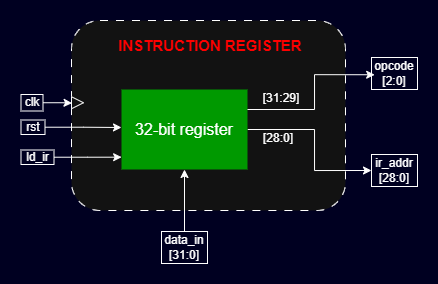
\includegraphics[width=0.65\textwidth]{Instruction_register.png} 
    \caption{Sơ đồ khối Instruction Register}
    \label{fig:ir_diagram}
\end{figure}

\textbf{Sơ đồ khối của Instruction Register gồm các thành phần giao tiếp chính:}

\begin{itemize}
    \item \textbf{Tín hiệu vào (Input):}
    \begin{itemize}
        \item \textbf{\texttt{data\_in [31:0]}:} Dữ liệu lệnh 32-bit nhận từ ngõ ra của bus bộ nhớ (Memory).
        \item \textbf{\texttt{ld\_ir}:} Tín hiệu cho phép nạp lệnh được cấp từ khối Controller. Lệnh mới chỉ được cập nhật vào thanh ghi khi tín hiệu này ở mức tích cực.
        \item \textbf{\texttt{rst}:} Tín hiệu reset đồng bộ (active high) để xóa câu lệnh hiện tại, đưa thanh ghi về trạng thái 0.
        \item \textbf{\texttt{clk}:} Xung lên của clk đồng bộ hóa quá trình lưu trữ dữ liệu.
    \end{itemize}
    
    \item \textbf{Tín hiệu ra (Output):}
    \begin{itemize}
        \item \textbf{\texttt{opcode [2:0]}:} 3-bit mã lệnh được trích xuất từ 3 bit cao nhất của thanh ghi (bit 31 đến 29). Tín hiệu này được gửi trực tiếp tới khối Controller để giải mã loại lệnh cần thực thi.
        \item \textbf{\texttt{ir\_addr [28:0]}:} 29-bit địa chỉ hoặc toán hạng được trích xuất từ phần còn lại của thanh ghi (bit 28 đến 0). Tín hiệu này được cấp cho khối Address Mux để định vị địa chỉ truy cập bộ nhớ trong giai đoạn Execute.
    \end{itemize}
\end{itemize}